\subsection{Utente Non Autenticato}
\subsubsection{UCW1 – Registrazione}
\begin{figure}[!h]
\centering
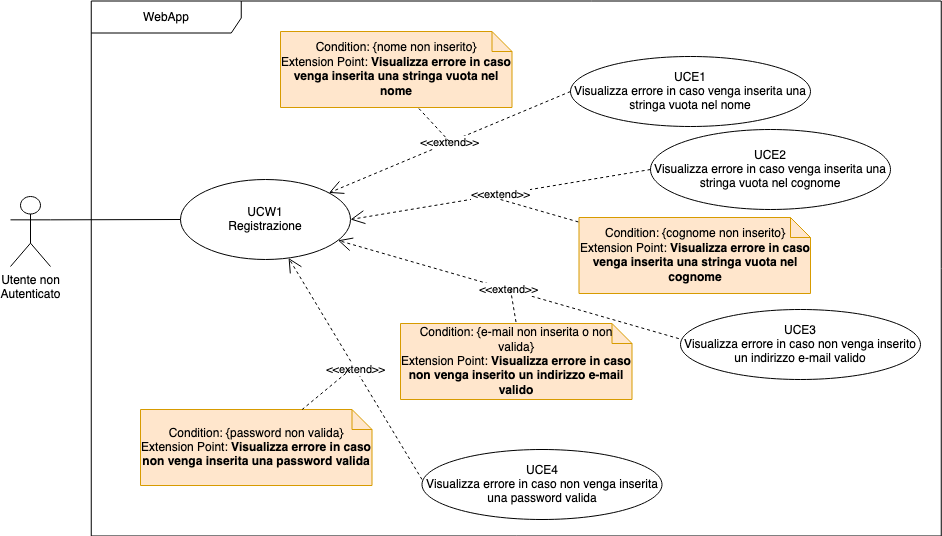
\includegraphics[scale=0.5]{UC_images/UCW1.png}
\caption{UCW1 – Registrazione}
\end{figure}
\begin{itemize}
\item \textbf{Descrizione}: L'utente non autenticato si registra nella piattaforma Sweeat.
\item \textbf{Attore primario}: Utente non autenticato.
\item \textbf{Precondizione}: L'utente non è ancora autenticato presso il sistema.
\item \textbf{Postcondizione}: L’utente possiede un account con cui può accedere alla piattaforma, contraddistinto da un indirizzo e-mail ed una password.

\item \textbf{Scenario principale}:
\begin{enumerate}
\item L’utente accede al sistema;
\item L’utente seleziona la funzionalità “Registrati”;
\item L'utente inserisce i campi dati obbligatori: Nome e Cognome;
\item L’utente inserisce un indirizzo e-mail univoco, non ancora utilizzato e con cui accedere alla piattaforma, nell'omonimo campo di registrazione; 
\item L’utente inserisce una password per accedere al sistema;
\item Affinché la registrazione vada a buon fine, l’utente dovrà cliccare su “Registrati”.
\end{enumerate}

\item \textbf{Estensioni}:
\begin{itemize}
\item Nel caso in cui l'utente non inserisca correttamente il suo nome
\begin{enumerate}
	\item L'utente non viene registrato nel sistema;
	\item Viene mostrato un messaggio d'errore che indica che il nome non è stato inserito correttamente (UCE1 §3.15).
\end{enumerate}
\item Nel caso in cui l'utente non inserisca correttamente il suo cognome
\begin{enumerate}
	\item L'utente non viene registrato nel sistema;
	\item Viene mostrato un messaggio d'errore che indica che il cognome non è stato inserito correttamente (UCE2 §3.16).
\end{enumerate}
\item Nel caso in cui l’utente inserisca un indirizzo e-mail non esistente, già presente a sistema o lasci il campo vuoto
\begin{enumerate}
	\item L’utente non viene registrato nel sistema;
	\item Viene mostrato un messaggio d’errore che indica che l'indirizzo e-mail inserito non è corretto (UCE3 §3.17).
\end{enumerate}
\item Nel caso in cui l’utente provi a registrarsi inserendo una password più breve di 8 caratteri
\begin{enumerate}
	\item L’utente non viene registrato nel sistema;
	\item Viene mostrato un messaggio d’errore che indica che non è stata inserita alcuna password (UCE4 §3.18).
\end{enumerate}
\end{itemize}
\end{itemize}